% Options for packages loaded elsewhere
\PassOptionsToPackage{unicode}{hyperref}
\PassOptionsToPackage{hyphens}{url}
%
\documentclass[
]{article}
\usepackage{amsmath,amssymb}
\usepackage{lmodern}
\usepackage{ifxetex,ifluatex}
\ifnum 0\ifxetex 1\fi\ifluatex 1\fi=0 % if pdftex
  \usepackage[T1]{fontenc}
  \usepackage[utf8]{inputenc}
  \usepackage{textcomp} % provide euro and other symbols
\else % if luatex or xetex
  \usepackage{unicode-math}
  \defaultfontfeatures{Scale=MatchLowercase}
  \defaultfontfeatures[\rmfamily]{Ligatures=TeX,Scale=1}
\fi
% Use upquote if available, for straight quotes in verbatim environments
\IfFileExists{upquote.sty}{\usepackage{upquote}}{}
\IfFileExists{microtype.sty}{% use microtype if available
  \usepackage[]{microtype}
  \UseMicrotypeSet[protrusion]{basicmath} % disable protrusion for tt fonts
}{}
\makeatletter
\@ifundefined{KOMAClassName}{% if non-KOMA class
  \IfFileExists{parskip.sty}{%
    \usepackage{parskip}
  }{% else
    \setlength{\parindent}{0pt}
    \setlength{\parskip}{6pt plus 2pt minus 1pt}}
}{% if KOMA class
  \KOMAoptions{parskip=half}}
\makeatother
\usepackage{xcolor}
\IfFileExists{xurl.sty}{\usepackage{xurl}}{} % add URL line breaks if available
\IfFileExists{bookmark.sty}{\usepackage{bookmark}}{\usepackage{hyperref}}
\hypersetup{
  pdftitle={Week 10 Quiz},
  pdfauthor={Michael Alford},
  hidelinks,
  pdfcreator={LaTeX via pandoc}}
\urlstyle{same} % disable monospaced font for URLs
\usepackage[margin=1in]{geometry}
\usepackage{color}
\usepackage{fancyvrb}
\newcommand{\VerbBar}{|}
\newcommand{\VERB}{\Verb[commandchars=\\\{\}]}
\DefineVerbatimEnvironment{Highlighting}{Verbatim}{commandchars=\\\{\}}
% Add ',fontsize=\small' for more characters per line
\usepackage{framed}
\definecolor{shadecolor}{RGB}{248,248,248}
\newenvironment{Shaded}{\begin{snugshade}}{\end{snugshade}}
\newcommand{\AlertTok}[1]{\textcolor[rgb]{0.94,0.16,0.16}{#1}}
\newcommand{\AnnotationTok}[1]{\textcolor[rgb]{0.56,0.35,0.01}{\textbf{\textit{#1}}}}
\newcommand{\AttributeTok}[1]{\textcolor[rgb]{0.77,0.63,0.00}{#1}}
\newcommand{\BaseNTok}[1]{\textcolor[rgb]{0.00,0.00,0.81}{#1}}
\newcommand{\BuiltInTok}[1]{#1}
\newcommand{\CharTok}[1]{\textcolor[rgb]{0.31,0.60,0.02}{#1}}
\newcommand{\CommentTok}[1]{\textcolor[rgb]{0.56,0.35,0.01}{\textit{#1}}}
\newcommand{\CommentVarTok}[1]{\textcolor[rgb]{0.56,0.35,0.01}{\textbf{\textit{#1}}}}
\newcommand{\ConstantTok}[1]{\textcolor[rgb]{0.00,0.00,0.00}{#1}}
\newcommand{\ControlFlowTok}[1]{\textcolor[rgb]{0.13,0.29,0.53}{\textbf{#1}}}
\newcommand{\DataTypeTok}[1]{\textcolor[rgb]{0.13,0.29,0.53}{#1}}
\newcommand{\DecValTok}[1]{\textcolor[rgb]{0.00,0.00,0.81}{#1}}
\newcommand{\DocumentationTok}[1]{\textcolor[rgb]{0.56,0.35,0.01}{\textbf{\textit{#1}}}}
\newcommand{\ErrorTok}[1]{\textcolor[rgb]{0.64,0.00,0.00}{\textbf{#1}}}
\newcommand{\ExtensionTok}[1]{#1}
\newcommand{\FloatTok}[1]{\textcolor[rgb]{0.00,0.00,0.81}{#1}}
\newcommand{\FunctionTok}[1]{\textcolor[rgb]{0.00,0.00,0.00}{#1}}
\newcommand{\ImportTok}[1]{#1}
\newcommand{\InformationTok}[1]{\textcolor[rgb]{0.56,0.35,0.01}{\textbf{\textit{#1}}}}
\newcommand{\KeywordTok}[1]{\textcolor[rgb]{0.13,0.29,0.53}{\textbf{#1}}}
\newcommand{\NormalTok}[1]{#1}
\newcommand{\OperatorTok}[1]{\textcolor[rgb]{0.81,0.36,0.00}{\textbf{#1}}}
\newcommand{\OtherTok}[1]{\textcolor[rgb]{0.56,0.35,0.01}{#1}}
\newcommand{\PreprocessorTok}[1]{\textcolor[rgb]{0.56,0.35,0.01}{\textit{#1}}}
\newcommand{\RegionMarkerTok}[1]{#1}
\newcommand{\SpecialCharTok}[1]{\textcolor[rgb]{0.00,0.00,0.00}{#1}}
\newcommand{\SpecialStringTok}[1]{\textcolor[rgb]{0.31,0.60,0.02}{#1}}
\newcommand{\StringTok}[1]{\textcolor[rgb]{0.31,0.60,0.02}{#1}}
\newcommand{\VariableTok}[1]{\textcolor[rgb]{0.00,0.00,0.00}{#1}}
\newcommand{\VerbatimStringTok}[1]{\textcolor[rgb]{0.31,0.60,0.02}{#1}}
\newcommand{\WarningTok}[1]{\textcolor[rgb]{0.56,0.35,0.01}{\textbf{\textit{#1}}}}
\usepackage{longtable,booktabs,array}
\usepackage{calc} % for calculating minipage widths
% Correct order of tables after \paragraph or \subparagraph
\usepackage{etoolbox}
\makeatletter
\patchcmd\longtable{\par}{\if@noskipsec\mbox{}\fi\par}{}{}
\makeatother
% Allow footnotes in longtable head/foot
\IfFileExists{footnotehyper.sty}{\usepackage{footnotehyper}}{\usepackage{footnote}}
\makesavenoteenv{longtable}
\usepackage{graphicx}
\makeatletter
\def\maxwidth{\ifdim\Gin@nat@width>\linewidth\linewidth\else\Gin@nat@width\fi}
\def\maxheight{\ifdim\Gin@nat@height>\textheight\textheight\else\Gin@nat@height\fi}
\makeatother
% Scale images if necessary, so that they will not overflow the page
% margins by default, and it is still possible to overwrite the defaults
% using explicit options in \includegraphics[width, height, ...]{}
\setkeys{Gin}{width=\maxwidth,height=\maxheight,keepaspectratio}
% Set default figure placement to htbp
\makeatletter
\def\fps@figure{htbp}
\makeatother
\setlength{\emergencystretch}{3em} % prevent overfull lines
\providecommand{\tightlist}{%
  \setlength{\itemsep}{0pt}\setlength{\parskip}{0pt}}
\setcounter{secnumdepth}{-\maxdimen} % remove section numbering
\ifluatex
  \usepackage{selnolig}  % disable illegal ligatures
\fi

\title{Week 10 Quiz}
\author{Michael Alford}
\date{}

\begin{document}
\maketitle

\textbf{Question 1}

Shown are four scatterplots. The calculated correlations are
\(0.008,\ -0.986,\ 0.671,\ -0.589\). Match the correlations to the
correct plot.

\begin{figure}
\centering
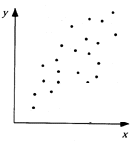
\includegraphics{/Users/malford/Documents/BPscyhSci/SIT191 - Statistics/Notes/Week 10/Week 10 Quiz/Images/scatter2a.png}
\caption{\(0.671\)}
\end{figure}

\begin{figure}
\centering
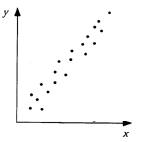
\includegraphics{/Users/malford/Documents/BPscyhSci/SIT191 - Statistics/Notes/Week 10/Week 10 Quiz/Images/scatter2b.png}
\caption{\(0.986\)}
\end{figure}

\begin{figure}
\centering
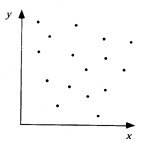
\includegraphics{/Users/malford/Documents/BPscyhSci/SIT191 - Statistics/Notes/Week 10/Week 10 Quiz/Images/scatter2c.png}
\caption{\(0.008\)}
\end{figure}

\begin{figure}
\centering
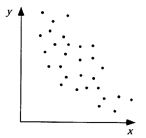
\includegraphics{/Users/malford/Documents/BPscyhSci/SIT191 - Statistics/Notes/Week 10/Week 10 Quiz/Images/scatter2d.png}
\caption{\(-0.589\)}
\end{figure}

\textbf{Question 2}

From the SPSS output below, what is the correlation value?

\begin{figure}
\centering
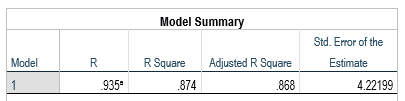
\includegraphics{/Users/malford/Documents/BPscyhSci/SIT191 - Statistics/Notes/Week 10/Week 10 Quiz/Images/corr 1.png}
\caption{corr1}
\end{figure}

\begin{itemize}
\tightlist
\item[$\square$]
  \(4.22199\)
\item[$\square$]
  \(87.4%
  \)
\item[$\boxtimes$]
  \(0.935\)
\item[$\square$]
  \(0.874\)
\item[$\square$]
  \(0.868\)
\end{itemize}

\textbf{Question 3}

For the following data, use SPSS or other technology to calculate the
correlation between the variables.

\begin{Shaded}
\begin{Highlighting}[]
\NormalTok{knitr}\SpecialCharTok{::}\FunctionTok{kable}\NormalTok{(Q3, }\StringTok{"pipe"}\NormalTok{)}
\end{Highlighting}
\end{Shaded}

\begin{longtable}[]{@{}rr@{}}
\toprule
x & y \\
\midrule
\endhead
15 & 24 \\
14 & 25 \\
17 & 21 \\
18 & 20 \\
14 & 26 \\
18 & 16 \\
19 & 19 \\
17 & 21 \\
15 & 22 \\
16 & 20 \\
\bottomrule
\end{longtable}

\begin{Shaded}
\begin{Highlighting}[]
\FunctionTok{round}\NormalTok{(}\FunctionTok{cor}\NormalTok{(Q3}\SpecialCharTok{$}\NormalTok{x, Q3}\SpecialCharTok{$}\NormalTok{y), }\DecValTok{3}\NormalTok{)}
\end{Highlighting}
\end{Shaded}

\begin{verbatim}
## [1] -0.867
\end{verbatim}

\begin{itemize}
\tightlist
\item[$\square$]
  \(-0.887\)
\item[$\square$]
  \(-887\)
\item[$\boxtimes$]
  \(-0.867\)
\item[$\square$]
  \(-0.786\)
\item[$\square$]
  \(0.87\)
\end{itemize}

\textbf{Question 4}

For a random sample of 15 adults, tibia length and height were recorded
with the SPSS linear regression analysis shown below. Researchers are
investigating whether tibia length can be used to predict height.

\begin{figure}
\centering
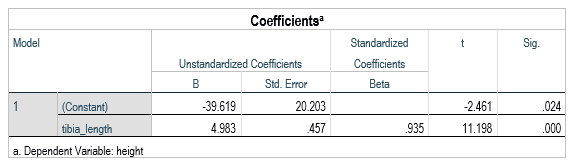
\includegraphics{/Users/malford/Documents/BPscyhSci/SIT191 - Statistics/Notes/Week 10/Week 10 Quiz/Images/tibia height.png}
\caption{Tibia Height}
\end{figure}

Which of the following gives the correct linear regression equation?

\begin{itemize}
\tightlist
\item[$\boxtimes$]
  \(\hat{height} = −39.619 + 4.983 \times tibia\)
\item[$\square$]
  \(\hat{height} = 39.619−4.983 \times tibia\)
\item[$\square$]
  \(\hat{tibia} = 4.983 \times height − 39.619\)
\item[$\square$]
  \(\hat{height} = −39.619 + 20.203 \times tibia\)
\item[$\square$]
  \(\hat{tibia} = 4.983 + 0.457 \times height\)
\end{itemize}

\textbf{Question 5}

Wild bears were caught and anesthetised so that various measurements
could be made. In particular, the usefulness of a bear's chest
circumference to predict its weight was of interest. A random sample of
10 bears was used, with the chest and weight measurements shown below,
as well as the linear regression analysis.

\begin{Shaded}
\begin{Highlighting}[]
\NormalTok{knitr}\SpecialCharTok{::}\FunctionTok{kable}\NormalTok{(Q5, }\StringTok{"pipe"}\NormalTok{)}
\end{Highlighting}
\end{Shaded}

\begin{longtable}[]{@{}rr@{}}
\toprule
Chest & Weight \\
\midrule
\endhead
26 & 80 \\
45 & 344 \\
54 & 416 \\
49 & 348 \\
35 & 166 \\
41 & 220 \\
41 & 262 \\
49 & 360 \\
38 & 204 \\
31 & 144 \\
\bottomrule
\end{longtable}

\begin{Shaded}
\begin{Highlighting}[]
\NormalTok{bearlm }\OtherTok{\textless{}{-}} \FunctionTok{lm}\NormalTok{(Weight }\SpecialCharTok{\textasciitilde{}}\NormalTok{ Chest, }\AttributeTok{data =}\NormalTok{ Q5)}
\FunctionTok{summary}\NormalTok{(bearlm)}
\end{Highlighting}
\end{Shaded}

\begin{verbatim}
## 
## Call:
## lm(formula = Weight ~ Chest, data = Q5)
## 
## Residuals:
##     Min      1Q  Median      3Q     Max 
## -35.638 -12.543   2.370   9.139  38.841 
## 
## Coefficients:
##              Estimate Std. Error t value Pr(>|t|)    
## (Intercept) -251.9479    33.8141  -7.451 7.26e-05 ***
## Chest         12.3801     0.8104  15.277 3.34e-07 ***
## ---
## Signif. codes:  0 '***' 0.001 '**' 0.01 '*' 0.05 '.' 0.1 ' ' 1
## 
## Residual standard error: 21.18 on 8 degrees of freedom
## Multiple R-squared:  0.9669, Adjusted R-squared:  0.9627 
## F-statistic: 233.4 on 1 and 8 DF,  p-value: 3.343e-07
\end{verbatim}

What can be said about the y-intercept (\(-251.948\)) in the context of
this study? (Select all that apply)

\begin{itemize}
\tightlist
\item[$\boxtimes$]
  The y-intercept would indicate the chest size of a bear with zero
  weight.
\item[$\square$]
  The y-intercept is close to a number of the observed data values and
  therefore seems reliable.
\item[$\square$]
  The y-intercept is meaningful in that it would represent the weight of
  bears when they are born.
\item[$\square$]
  The y-intercept would indicate the weight of a bear with zero chest
  circumference.\\
\item[$\boxtimes$]
  The y-intercept is based on extrapolation and therefore is not
  reliable.
\item[$\boxtimes$]
  The y-intercept is not meaningful for this data as it would not make
  sense to have a bear with zero chest size or negative weight.
\end{itemize}

\textbf{Question 6}

For a random sample of 15 adults, tibia (shinbone) length and height
were recorded (in cm) with the SPSS linear regression analysis shown
below. Researchers are investigating whether tibia length can be used to
predict height.

\begin{figure}
\centering
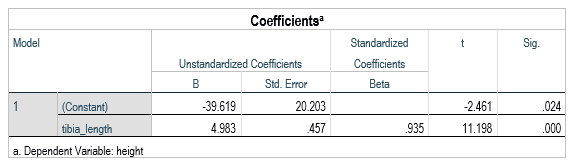
\includegraphics{/Users/malford/Documents/BPscyhSci/SIT191 - Statistics/Notes/Week 10/Week 10 Quiz/Images/tibia height.png}
\caption{tibia height}
\end{figure}

Which option is the correct interpretation of the slope of the
regression equation?

\begin{itemize}
\tightlist
\item[$\square$]
  An increase in tibia length of 1cm corresponds with an increase in
  height of 4.983cm.
\item[$\boxtimes$]
  An increase in height of 1cm corresponds with an increase in tibia
  length of 4.983cm.
\item[$\square$]
  An increase in tibia length of 1cm corresponds with an increase in
  height of 39.619cm.
\item[$\square$]
  A decrease in tibia length of 39.619cm corresponds with an increase in
  height of 4.983cm.
\item[$\square$]
  An increase in tibia length of 1cm corresponds with a decrease in
  height of 4.983cm.
\end{itemize}

\textbf{Question 7}

For the following data, use SPSS to calculate the regression equation to
predict y from x, then select the correct answer.

\begin{Shaded}
\begin{Highlighting}[]
\NormalTok{knitr}\SpecialCharTok{::}\FunctionTok{kable}\NormalTok{(Q7, }\StringTok{"pipe"}\NormalTok{)}
\end{Highlighting}
\end{Shaded}

\begin{longtable}[]{@{}rr@{}}
\toprule
x & y \\
\midrule
\endhead
15 & 20 \\
14 & 19 \\
17 & 23 \\
18 & 24 \\
14 & 17 \\
18 & 24 \\
19 & 26 \\
17 & 22 \\
15 & 18 \\
16 & 20 \\
\bottomrule
\end{longtable}

\begin{Shaded}
\begin{Highlighting}[]
\NormalTok{Q7lm }\OtherTok{\textless{}{-}} \FunctionTok{lm}\NormalTok{(y }\SpecialCharTok{\textasciitilde{}}\NormalTok{ x, }\AttributeTok{data =}\NormalTok{ Q7)}
\FunctionTok{summary}\NormalTok{(Q7lm)}
\end{Highlighting}
\end{Shaded}

\begin{verbatim}
## 
## Call:
## lm(formula = y ~ x, data = Q7)
## 
## Residuals:
##      Min       1Q   Median       3Q      Max 
## -1.21352 -0.56228 -0.02847  0.52402  1.39146 
## 
## Coefficients:
##             Estimate Std. Error t value Pr(>|t|)    
## (Intercept)  -4.8612     2.6127  -1.861   0.0998 .  
## x             1.6050     0.1594  10.066 8.08e-06 ***
## ---
## Signif. codes:  0 '***' 0.001 '**' 0.01 '*' 0.05 '.' 0.1 ' ' 1
## 
## Residual standard error: 0.8452 on 8 degrees of freedom
## Multiple R-squared:  0.9268, Adjusted R-squared:  0.9177 
## F-statistic: 101.3 on 1 and 8 DF,  p-value: 8.082e-06
\end{verbatim}

\begin{itemize}
\tightlist
\item[$\square$]
  \(\hat{y} = −6.283 + 0.533x\)
\item[$\boxtimes$]
  \(\hat{y} = −4.861 + 1.605x\)
\item[$\square$]
  \(\hat{y} = 1.605 − 4.861x\)
\item[$\square$]
  \(\hat{y} = 12.794 − 1.715x\)
\item[$\square$]
  \(\hat{y} = 4 + 0.577x\)
\end{itemize}

\textbf{Question 8}

Information on a number of flights from a particular airport was
gathered, including the distance of the flight and how much it cost.
Using this data, a scatterplot was generated along with a regression
model.

\begin{Shaded}
\begin{Highlighting}[]
\NormalTok{knitr}\SpecialCharTok{::}\FunctionTok{kable}\NormalTok{(Q8, }\StringTok{"pipe"}\NormalTok{)}
\end{Highlighting}
\end{Shaded}

\begin{longtable}[]{@{}rr@{}}
\toprule
Distance & Cost \\
\midrule
\endhead
568 & 219 \\
933 & 222 \\
720 & 249 \\
1190 & 308 \\
602 & 249 \\
683 & 240 \\
1719 & 252 \\
589 & 229 \\
327 & 183 \\
894 & 209 \\
419 & 199 \\
749 & 248 \\
749 & 301 \\
392 & 238 \\
657 & 205 \\
461 & 232 \\
1565 & 374 \\
2150 & 343 \\
\bottomrule
\end{longtable}

\begin{Shaded}
\begin{Highlighting}[]
\NormalTok{Q8lm }\OtherTok{\textless{}{-}} \FunctionTok{lm}\NormalTok{(Cost }\SpecialCharTok{\textasciitilde{}}\NormalTok{ Distance, }\AttributeTok{data =}\NormalTok{ Q8)}
\FunctionTok{summary}\NormalTok{(Q8lm)}
\end{Highlighting}
\end{Shaded}

\begin{verbatim}
## 
## Call:
## lm(formula = Cost ~ Distance, data = Q8)
## 
## Residuals:
##     Min      1Q  Median      3Q     Max 
## -62.994 -25.164   0.854  16.305  70.574 
## 
## Coefficients:
##              Estimate Std. Error t value Pr(>|t|)    
## (Intercept) 185.87405   16.81114  11.057 6.67e-09 ***
## Distance      0.07511    0.01713   4.384 0.000462 ***
## ---
## Signif. codes:  0 '***' 0.001 '**' 0.01 '*' 0.05 '.' 0.1 ' ' 1
## 
## Residual standard error: 35.16 on 16 degrees of freedom
## Multiple R-squared:  0.5457, Adjusted R-squared:  0.5174 
## F-statistic: 19.22 on 1 and 16 DF,  p-value: 0.000462
\end{verbatim}

\begin{Shaded}
\begin{Highlighting}[]
\FunctionTok{plot}\NormalTok{(Q8}\SpecialCharTok{$}\NormalTok{Distance }\SpecialCharTok{\textasciitilde{}}\NormalTok{ Q8}\SpecialCharTok{$}\NormalTok{Cost, }\AttributeTok{xlab =} \StringTok{"Distance (km)"}\NormalTok{, }\AttributeTok{ylab =} \StringTok{"Cost ($)"}\NormalTok{)}
\FunctionTok{abline}\NormalTok{(Q8lm)}
\end{Highlighting}
\end{Shaded}

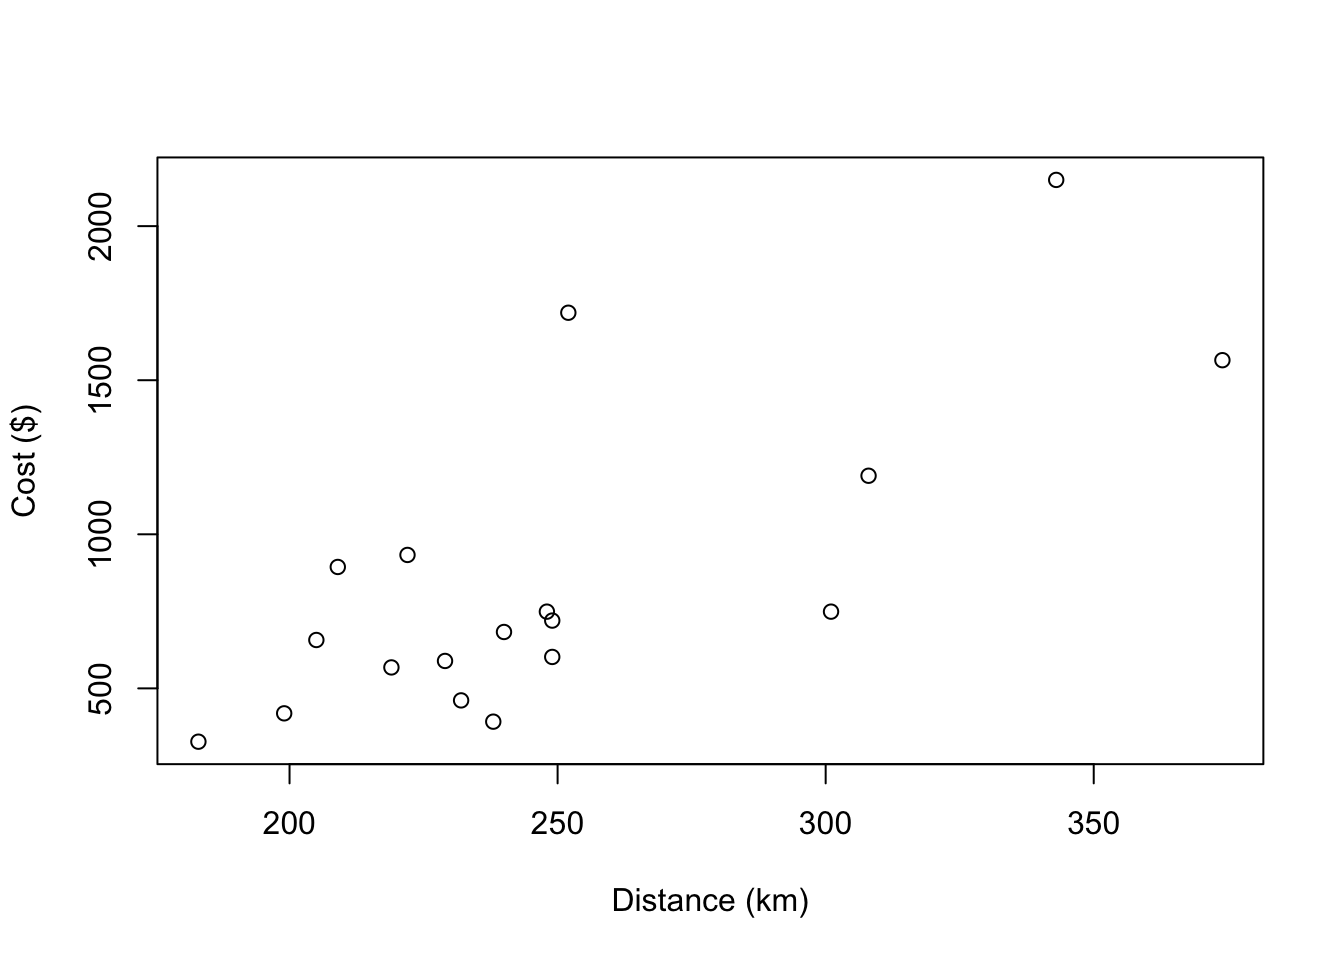
\includegraphics{Week-10-Quiz_files/figure-latex/unnamed-chunk-4-1.pdf}

Based on this, indicate your answers to the following questions.

\begin{enumerate}
\def\labelenumi{\alph{enumi}.}
\tightlist
\item
  The explanatory variable is
\end{enumerate}

\begin{itemize}
\tightlist
\item[$\boxtimes$]
  Distance
\item[$\square$]
  Cost
\end{itemize}

\begin{enumerate}
\def\labelenumi{\alph{enumi}.}
\setcounter{enumi}{1}
\tightlist
\item
  The response variable is
\end{enumerate}

\begin{itemize}
\tightlist
\item[$\square$]
  Distance
\item[$\boxtimes$]
  Cost
\end{itemize}

\begin{enumerate}
\def\labelenumi{\alph{enumi}.}
\setcounter{enumi}{2}
\tightlist
\item
  Based on the scatterplot, is the relationship:
\end{enumerate}

\begin{itemize}
\tightlist
\item[$\boxtimes$]
  positive
\item[$\square$]
  negative
\end{itemize}

\begin{enumerate}
\def\labelenumi{\alph{enumi}.}
\setcounter{enumi}{3}
\tightlist
\item
  Give the correlation of distance with cost. (give your answer to 3
  decimal places, e.g.~\(0.453\ or\ -0.453\) if the relationship is
  negative)
\end{enumerate}

\begin{Shaded}
\begin{Highlighting}[]
  \FunctionTok{round}\NormalTok{(}\FunctionTok{cor}\NormalTok{(Q8}\SpecialCharTok{$}\NormalTok{Distance, Q8}\SpecialCharTok{$}\NormalTok{Cost), }\DecValTok{3}\NormalTok{)}
\end{Highlighting}
\end{Shaded}

\begin{verbatim}
## [1] 0.739
\end{verbatim}

\begin{enumerate}
\def\labelenumi{\alph{enumi}.}
\setcounter{enumi}{4}
\tightlist
\item
  What is the \(R^2\) value? (give your answer as a percentage to 1
  decimal place, e.g.~23.1, without the \% sign)
\end{enumerate}

\begin{itemize}
\tightlist
\item[$\boxtimes$]
  54.6
\end{itemize}

\begin{enumerate}
\def\labelenumi{\alph{enumi}.}
\setcounter{enumi}{5}
\tightlist
\item
  The linear equation you would use to estimate the cost from distance
  is \(\hat{y} = a + bx\) where:
\end{enumerate}

\begin{itemize}
\tightlist
\item[$\square$]
  \(a\) is 0.739 and \(b\) is 0.564
\item[$\square$]
  \(a\) is 185.874 and \(b\) is 16.811
\item[$\boxtimes$]
  \(a\) is 185.874 and \(b\) is 0.075
\item[$\square$]
  \(a\) is 35.16288 and \(b\) is 185.874
\end{itemize}

\begin{enumerate}
\def\labelenumi{\alph{enumi}.}
\setcounter{enumi}{6}
\tightlist
\item
  Use the equation to predict the cost of a flight that is 800km. (give
  your answer to 2 decimal places without the \$ sign)
\end{enumerate}

\[
  \begin{aligned}
    \hat{y} &= a + bx\\
    &= 185.874 + 0.075 \times 800\\
    &= 245.87
  \end{aligned}
\]

\begin{enumerate}
\def\labelenumi{\alph{enumi}.}
\setcounter{enumi}{7}
\tightlist
\item
  Is this answer:
\end{enumerate}

\begin{itemize}
\tightlist
\item[$\boxtimes$]
  reliable because it is not based on extrapolation or
\item[$\square$]
  unreliable because it is based on extrapolation?
\end{itemize}

\textbf{Question 9}

For a random sample of 15 adults, tibia (shinbone) length and height
were recorded with the SPSS linear regression analysis given below.
Researchers are investigating whether tibia length can be used to
predict height.

\begin{figure}
\centering
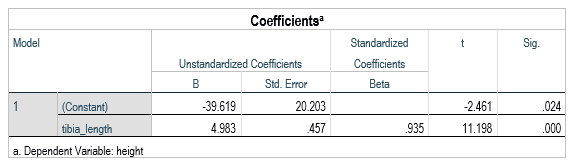
\includegraphics{/Users/malford/Documents/BPscyhSci/SIT191 - Statistics/Notes/Week 10/Week 10 Quiz/Images/tibia height.png}
\caption{Tibia Height}
\end{figure}

Is the relationship between tibia length and height significant using
\(\alpha = 0.01\)? Select the correct option.

\begin{itemize}
\tightlist
\item[$\square$]
  \(t = 11.198\ and\ P = 0.000\) so the relationship is significant
\item[$\boxtimes$]
  \(t = 11.198\ and\ P = 0.000\) so the relationship is not significant
\item[$\square$]
  \(t = 11.198\ and\ P = 0.024\) so the relationship is not significant
\item[$\square$]
  \(t = -2.461\ and\ P = 0.024\) so the relationship is not significant
\item[$\square$]
  \(t = -2.461\ and\ P = 0.012\) so the relationship is significant
\end{itemize}

\textbf{Question 10}

For the following data, use SPSS to obtain the regression output to
predict y from x.

\begin{Shaded}
\begin{Highlighting}[]
\NormalTok{knitr}\SpecialCharTok{::}\FunctionTok{kable}\NormalTok{(Q10, }\StringTok{"pipe"}\NormalTok{)}
\end{Highlighting}
\end{Shaded}

\begin{longtable}[]{@{}rr@{}}
\toprule
x & y \\
\midrule
\endhead
15 & 20 \\
14 & 19 \\
17 & 23 \\
18 & 24 \\
14 & 17 \\
18 & 24 \\
19 & 26 \\
17 & 22 \\
15 & 18 \\
16 & 20 \\
\bottomrule
\end{longtable}

\begin{Shaded}
\begin{Highlighting}[]
\NormalTok{Q10lm }\OtherTok{\textless{}{-}} \FunctionTok{lm}\NormalTok{(y }\SpecialCharTok{\textasciitilde{}}\NormalTok{ x, }\AttributeTok{data =}\NormalTok{ Q10)}
\FunctionTok{summary}\NormalTok{(Q10lm)}
\end{Highlighting}
\end{Shaded}

\begin{verbatim}
## 
## Call:
## lm(formula = y ~ x, data = Q10)
## 
## Residuals:
##      Min       1Q   Median       3Q      Max 
## -1.21352 -0.56228 -0.02847  0.52402  1.39146 
## 
## Coefficients:
##             Estimate Std. Error t value Pr(>|t|)    
## (Intercept)  -4.8612     2.6127  -1.861   0.0998 .  
## x             1.6050     0.1594  10.066 8.08e-06 ***
## ---
## Signif. codes:  0 '***' 0.001 '**' 0.01 '*' 0.05 '.' 0.1 ' ' 1
## 
## Residual standard error: 0.8452 on 8 degrees of freedom
## Multiple R-squared:  0.9268, Adjusted R-squared:  0.9177 
## F-statistic: 101.3 on 1 and 8 DF,  p-value: 8.082e-06
\end{verbatim}

Is there a significant relationship between the variables at
\(\alpha = 0.05\)? From your output, select the test statistic value and
P for this hypothesis test.

\begin{itemize}
\tightlist
\item[$\square$]
  \(t = 3.246\ and\ P = 0.012\) (significant relationship)
\item[$\square$]
  \(t = -1.861\ and\ P = 0.100\) (no significant relationship)
\item[$\square$]
  \(t = 10.066\ and\ P = 0.100\) (no significant relationship)
\item[$\square$]
  \(t = 10.066\ and\ P = 0.05\) (no significant relationship)
\item[$\boxtimes$]
  \(t = 10.066\ and\ P < 0.001\) (significant relationship)
\end{itemize}

\end{document}
